% Черновик по редакционному шаблону СибЖИМ; сведения об авторах, УДК и финансировании необходимо дополнить.
% Для локального предпросмотра в копии класса изменён только графический драйвер.
\documentclass[notitle]{sibjima_preview}
\usepackage{fontspec}
\setmainfont{cmunrm.otf}[BoldFont=cmunbx.otf,ItalicFont=cmunti.otf,BoldItalicFont=cmunbi.otf]
\usepackage{booktabs,array}
\usepackage[hidelinks]{hyperref}
\newcommand{\ii}{\mathrm{i}}
\newcommand{\R}{\mathbb{R}}
\begin{document}
\thispagestyle{plain}
\pagestyle{plain}
\begin{center}
{\bfseries Приближённое решение задачи рассеяния для уравнения Гельмгольца на основе SVD и спектрального нейрооператора}
\end{center}

\textbf{Аннотация:} Рассматривается двумерная задача рассеяния плоской волны на неоднородных круглых включениях. Исследуется схема приближённого вычисления комплексного рассеянного поля по коэффициентам среды, направлению падающей волны и волновому числу. Обучающая выборка формируется методом конечных элементов на общей неструктурированной треугольной сетке. Для понижения размерности входных данных и решения используется приближённое сингулярное разложение матриц снимков. Нелинейное отображение между коэффициентами разложения аппроксимируется спектральным нейрооператором. Число сохраняемых мод выбирается по ошибке восстановления на валидационной выборке. По сохранённой истории обучения за первые 500 эпох наименьшая средняя относительная узловая ошибка на валидационной выборке составила около 7,06 процента. Тестовая ошибка модели, выбранной в пределах этих эпох, пока не оценена.

\textbf{Ключевые слова}: уравнение Гельмгольца; рассеяние волн; метод конечных элементов; сингулярное разложение; понижение размерности; спектральный нейрооператор.

\section{ВВЕДЕНИЕ}
При решении серии задач рассеяния приходится многократно вычислять волновое поле при изменении коэффициентов среды и параметров падающей волны. Один из подходов к построению приближённого решения состоит в обучении отображения между параметрами задачи и решением. Нейрооператорные модели используют для этого функциональные представления входных данных и выходного поля~\cite{li2020}. В спектральном подходе нелинейное отображение может задаваться непосредственно между коэффициентами разложений по выбранным базисам~\cite{fanaskov2022}.

Цель работы состоит в построении и исследовании приближённого оператора решения двумерной задачи рассеяния с использованием конечно-элементных данных и сингулярного разложения. Пространственные базисы полей определяются по обучающей выборке; нелинейное отображение между коэффициентами разложения задаётся нейросетью. Для всех примеров используется одна фиксированная сетка. В работе рассматриваются выбор числа сохраняемых мод и точность приближения на валидационной выборке.

\section{ПОСТАНОВКА ЗАДАЧИ}
Пусть \(\Omega=(-2,2)^2\subset\R^2\) --- расчётная область. Падающая плоская волна задаётся выражением
\begin{equation*}
u_i(\bm{x})=\exp\!\bigl(\ii k\,\bm{d}\cdot\bm{x}\bigr),
\qquad
\bm{d}=(\cos\theta,\sin\theta),\quad k>0.
\end{equation*}
Требуется найти комплексное рассеянное поле \(u_s(\bm{x})\), удовлетворяющее уравнению
\begin{equation}
\nabla\cdot(A\nabla u_s)+k^2n u_s
=
\nabla\cdot\bigl((1-A)\nabla u_i\bigr)+k^2(1-n)u_i,
\qquad \bm{x}\in\Omega,
\tag{1}\label{eq:helmholtz}
\end{equation}
с поглощающим граничным условием
\begin{equation}
A\frac{\partial u_s}{\partial\nu}=\ii k u_s,
\qquad \bm{x}\in\partial\Omega,
\tag{2}\label{eq:boundary}
\end{equation}
где \(\nu\) --- внешняя единичная нормаль. Предполагается, что включения расположены внутри области и \(A=1\) в окрестности \(\partial\Omega\). Полное поле определяется как \(u=u_i+u_s\).

Коэффициенты \(A(\bm{x})\) и \(n(\bm{x})\) принимают постоянные значения внутри включений и равны единице вне их. Включения выбираются из фиксированного набора 24 кругов. Для каждой среды активируются от 3 до 10 кругов; значения коэффициентов внутри активных включений принадлежат диапазонам
\begin{equation}
0{,}6\leq A_{\mathrm{in}}\leq0{,}9,\qquad
1{,}5\leq n_{\mathrm{in}}\leq3,\qquad
1\leq k\leq2.
\tag{3}\label{eq:ranges}
\end{equation}
Коэффициенты включений выбираются по логарифмически равномерному распределению, волновое число --- по равномерному распределению.

Таким образом, рассматривается приближение отображения
\begin{equation*}
\mathcal{G}:(A,n,\theta,k)\longmapsto u_s.
\end{equation*}
Условие~\eqref{eq:boundary} задаёт модель на конечной расчётной области. Погрешность замены внешней задачи этим условием отдельно не исследуется.

\section{КОНЕЧНО-ЭЛЕМЕНТНАЯ ДИСКРЕТИЗАЦИЯ}
В области \(\Omega\) строится общая неструктурированная треугольная сетка, согласованная с границами всех возможных включений. Коэффициенты \(A\) и \(n\) задаются как кусочно-постоянные функции по элементам. Для решения используется пространство непрерывных кусочно-линейных комплекснозначных функций \(V_h\).

Умножим~\eqref{eq:helmholtz} на комплексно-сопряжённую пробную функцию \(\overline{v_h}\), проинтегрируем по частям и учтём~\eqref{eq:boundary}. Получим задачу: найти \(u_{s,h}\in V_h\), для которого
\begin{align*}
&\int_\Omega A\nabla u_{s,h}\cdot\nabla\overline{v_h}\,d\bm{x}
-k^2\int_\Omega n u_{s,h}\overline{v_h}\,d\bm{x}
-\ii k\int_{\partial\Omega}u_{s,h}\overline{v_h}\,ds
\nonumber\\
&\qquad =
-\int_\Omega(A-1)\nabla u_i\cdot\nabla\overline{v_h}\,d\bm{x}
+k^2\int_\Omega(n-1)u_i\overline{v_h}\,d\bm{x},
\qquad \forall v_h\in V_h.
\end{align*}
Возникающая система линейных алгебраических уравнений решается прямым методом.

В вычислительном эксперименте целевой шаг фоновой сетки составляет \(h\approx4/96\). Сетка содержит 11\,380 узлов и 22\,374 треугольных элемента. Для передачи коэффициентов среды в модель выполняется усреднение значений соседних элементов в узлах. Это усреднение используется при построении SVD-представления; конечно-элементный расчёт выполняется с исходными поэлементными коэффициентами.

\section{SVD-ПРЕДСТАВЛЕНИЕ КОЭФФИЦИЕНТОВ И РЕШЕНИЯ}
Пусть \(\bm{f}^{(s)}\in\R^{N_h}\), \(s=1,\ldots,N_{\mathrm{tr}}\), --- узловые векторы некоторого вещественного поля на обучающей выборке. Введём среднее поле
\begin{equation*}
\overline{\bm{f}}=\frac{1}{N_{\mathrm{tr}}}\sum_{s=1}^{N_{\mathrm{tr}}}\bm{f}^{(s)}
\end{equation*}
и матрицу центрированных снимков. Для точного сингулярного разложения имеем
\begin{equation*}
F_c=
\begin{bmatrix}
(\bm{f}^{(1)}-\overline{\bm{f}})^\mathsf{T}\\
\vdots\\
(\bm{f}^{(N_{\mathrm{tr}})}-\overline{\bm{f}})^\mathsf{T}
\end{bmatrix}
=U\Sigma V^\mathsf{T}.
\end{equation*}
Первые \(R\) правых сингулярных векторов образуют матрицу пространственного базиса
\(\Phi_R=[\bm{\phi}_1,\ldots,\bm{\phi}_R]\in\R^{N_h\times R}\). Тогда
\begin{equation*}
\bm{f}^{(s)}\approx
\overline{\bm{f}}+\Phi_R\bm{C}^{(s)},\qquad
\bm{C}^{(s)}=\Phi_R^\mathsf{T}
(\bm{f}^{(s)}-\overline{\bm{f}}).
\end{equation*}
Здесь \(R\) --- число сохраняемых мод, а \(C_j^{(s)}\) --- вес \(j\)-й моды для \(s\)-го примера. Следовательно, коэффициенты \(\bm{C}^{(s)}\) являются компактным представлением поля. Для обучающей выборки матрица коэффициентов в случае точного разложения имеет вид
\begin{equation}
C=F_c\Phi_R=U_R\Sigma_R.
\tag{4}\label{eq:matrix_coefficients}
\end{equation}

Отдельные базисы строятся для \(A\), \(n\), \(\operatorname{Re}u_s\) и \(\operatorname{Im}u_s\). Для \(A\) и \(n\) используется по одному снимку на физическую среду, поскольку смена направления падающей волны не меняет коэффициенты среды. В вычислениях базисы строятся с помощью рандомизированной схемы с дополнительными векторами и степенными итерациями~\cite{halko2011}. Поэтому равенство \(C=F_c\Phi_R\) используется как определение коэффициентов для полученного приближённого базиса, тогда как представление через точные сингулярные множители в~\eqref{eq:matrix_coefficients} относится к точному SVD.

В данной реализации ортогональность базиса определяется евклидовым скалярным произведением узловых векторов. Оно отличается от скалярного произведения с конечно-элементной матрицей масс. Поэтому ниже отдельно приводятся узловая и интегральная ошибки.

\section{ВЫБОР ЧИСЛА МОД И НОРМИРОВКА}
Ранг выбирается по ошибке восстановления решения на валидационной выборке:
\begin{equation*}
R_*=\min\left\{r:
\frac{1}{N_{\mathrm{val}}}\sum_{s=1}^{N_{\mathrm{val}}}
\frac{\|\bm{u}^{(s)}-\bm{u}_r^{(s)}\|_2}
{\|\bm{u}^{(s)}\|_2}
\leq\varepsilon_{\mathrm{POD}}\right\}.
\end{equation*}
При этом базисы определяются по обучающей выборке; тестовые данные при выборе ранга не используются. Для допуска \(\varepsilon_{\mathrm{POD}}=10^{-2}\) получено \(R_*=71\). Средняя ошибка восстановления на валидации составила около \(0{,}970\%\), её 95-й процентиль --- около \(2{,}31\%\). Данный критерий ограничивает среднюю ошибку и не задаёт одинаковой точности для каждого примера.

Поскольку геометрия включений фиксирована, центрированные поля \(A\) и \(n\) принадлежат пространству, порождённому индикаторами 24 кругов. Их значимая численная размерность не превышает 24. Столбцы входных базисов, отвечающие численно нулевым сингулярным значениям, зануляются. Это исключает усиление ошибок округления при нормировке малых коэффициентов.

Для каждой сохранённой компоненты используется нормировка
\begin{equation*}
\widetilde C_j^{(s)}
=\frac{C_j^{(s)}-\mu_j}{\sigma_j},
\end{equation*}
где \(\mu_j\) и \(\sigma_j\) --- среднее и стандартное отклонение, вычисленные по обучающей выборке. Для компоненты с нулевым или численно малым отклонением вместо \(\sigma_j\) в знаменателе используется единица. Неактивные входные компоненты остаются равными нулю.

\section{ОТОБРАЖЕНИЕ В ПРОСТРАНСТВЕ КОЭФФИЦИЕНТОВ}
Нейросеть аппроксимирует отображение
\begin{equation*}
\mathcal{N}_{\bm{\eta}}:
(\widetilde{\bm{C}}_A,\widetilde{\bm{C}}_n,\cos\theta,\sin\theta,\widetilde{k})
\longmapsto
(\widehat{\widetilde{\bm{C}}}_{r},\widehat{\widetilde{\bm{C}}}_{i}),
\end{equation*}
где \(\bm{\eta}\) --- обучаемые параметры. Каждой моде соответствует входной вектор из пяти компонент. Параметры направления и нормированное волновое число повторяются для всех мод.

После начального линейного преобразования используются четыре слоя с шириной 64 и активацией GELU. Слой содержит преобразование каналов и смешивание пространственных мод:
\begin{equation*}
Z^{(\ell+1)}
=
Z^{(\ell)}
+\sigma\!\left(
Z^{(\ell)}W_{\mathrm{loc}}^{(\ell)}
+B^{(\ell)}Z^{(\ell)}W_{\mathrm{ch}}^{(\ell)}
+b^{(\ell)}\right),
\end{equation*}
где \(Z^{(\ell)}\in\R^{R\times64}\),
\(B^{(\ell)}\in\R^{R\times R}\).
Линейная выходная проекция даёт нормированные коэффициенты действительной и мнимой частей решения. При \(R=71\) модель содержит 53\,958 обучаемых параметров.

После обратной нормировки поле восстанавливается по формуле
\begin{equation*}
\widehat{\bm{u}}_s=
\overline{\bm{u}}_r+\Phi_r\widehat{\bm{C}}_r
+\ii\bigl(\overline{\bm{u}}_i+\Phi_i\widehat{\bm{C}}_i\bigr).
\end{equation*}
Таким образом, нейросеть предсказывает коэффициенты разложения, а пространственная зависимость задаётся предварительно построенными базисами.

\section{ОБУЧЕНИЕ И ОЦЕНКА ПОГРЕШНОСТИ}
В обучении учитывается исходный масштаб выходных коэффициентов. Для одного примера введём остаток SVD-проекции
\(\bm{\rho}^{(s)}=\bm{u}^{(s)}-\bm{u}_R^{(s)}\).
При ортонормированных базисах узловая ошибка представляется в виде
\begin{equation}
\|\widehat{\bm{u}}^{(s)}-\bm{u}^{(s)}\|_2^2
=
\|\widehat{\bm{C}}_r^{(s)}-\bm{C}_r^{(s)}\|_2^2
+\|\widehat{\bm{C}}_i^{(s)}-\bm{C}_i^{(s)}\|_2^2
+\|\bm{\rho}^{(s)}\|_2^2.
\tag{5}\label{eq:error_decomposition}
\end{equation}
Функция потерь определяется средним относительным значением нормы из~\eqref{eq:error_decomposition}. Использование только нормированных коэффициентов с одинаковыми весами изменило бы вклад отдельных мод в ошибку поля.

Минимизация функции потерь проводится на обучающей выборке методом Adam с начальным шагом \(10^{-3}\) и размером пакета 256. Шаг уменьшается вдвое через каждые 100 эпох до значения \(10^{-5}\). Валидационная выборка используется для контроля обучения и выбора модели; в обновлении параметров она не участвует. Для контроля остановки используется отсутствие улучшения более чем на \(10^{-4}\) в течение 80 эпох после первых 100 эпох. Предельное число эпох принято равным 500. Достижение этого предела рассматривается отдельно от остановки по указанному критерию.

Для итоговой оценки используются две характеристики:
\begin{equation*}
e_{\mathrm{node}}^{(s)}
=\frac{\|\widehat{\bm{u}}^{(s)}-\bm{u}^{(s)}\|_2}
{\|\bm{u}^{(s)}\|_2},\qquad
e_{L^2}^{(s)}
=\left(
\frac{(\widehat{\bm{u}}^{(s)}-\bm{u}^{(s)})^*M
(\widehat{\bm{u}}^{(s)}-\bm{u}^{(s)})}
{(\bm{u}^{(s)})^*M\bm{u}^{(s)}}
\right)^{1/2},
\end{equation*}
где \(M\) --- согласованная матрица масс. Для линейного треугольного элемента \(T\) локальная матрица масс равна
\begin{equation*}
M_T=\frac{|T|}{12}
\begin{pmatrix}2&1&1\\1&2&1\\1&1&2\end{pmatrix}.
\end{equation*}

\section{ЧИСЛЕННЫЙ ЭКСПЕРИМЕНТ}
Сформирована выборка из 1000 сред. Для каждой среды рассматриваются восемь равномерно расположенных направлений падающей волны со случайным общим угловым сдвигом. Всего получено 8000 решений. Обучающая, валидационная и тестовая выборки содержат соответственно 6400, 800 и 800 примеров, то есть 800, 100 и 100 различных сред. Все направления одной среды относятся к одной выборке.

В таблице~\ref{tab:results} приведены характеристики первых 500 эпох сохранённой истории обучения. Наименьшая валидационная ошибка за этот интервал достигнута на 492-й эпохе. Эти данные получены из истории более продолжительного запуска; отдельный запуск с пределом 500 эпох и тестирование соответствующей модели ещё не выполнены. Достижение сходимости по критерию отсутствия улучшения не утверждается.
\begin{table}[htbp]
\centering
\caption{Характеристики обучения в пределах 500 эпох, \(R=71\)}
\label{tab:results}
\begin{tabular}{@{}lr@{}}
\toprule
Характеристика & Значение\\
\midrule
Число рассматриваемых эпох & 500\\
Эпоха наименьшей валидационной ошибки & 492\\
Наименьшая валидационная узловая ошибка, \% & 7,061\\
Валидационная узловая ошибка на 500-й эпохе, \% & 7,064\\
\bottomrule
\end{tabular}
\end{table}

На рис.~\ref{fig:training} представлены значения функции потерь в пределах первых 500 эпох. Обучающее значение усредняется по пакетам в процессе обновления параметров, валидационное вычисляется по фиксированной модели в конце эпохи. После начального снижения уменьшение валидационной ошибки замедляется.
\begin{figure}[htbp]
\centering
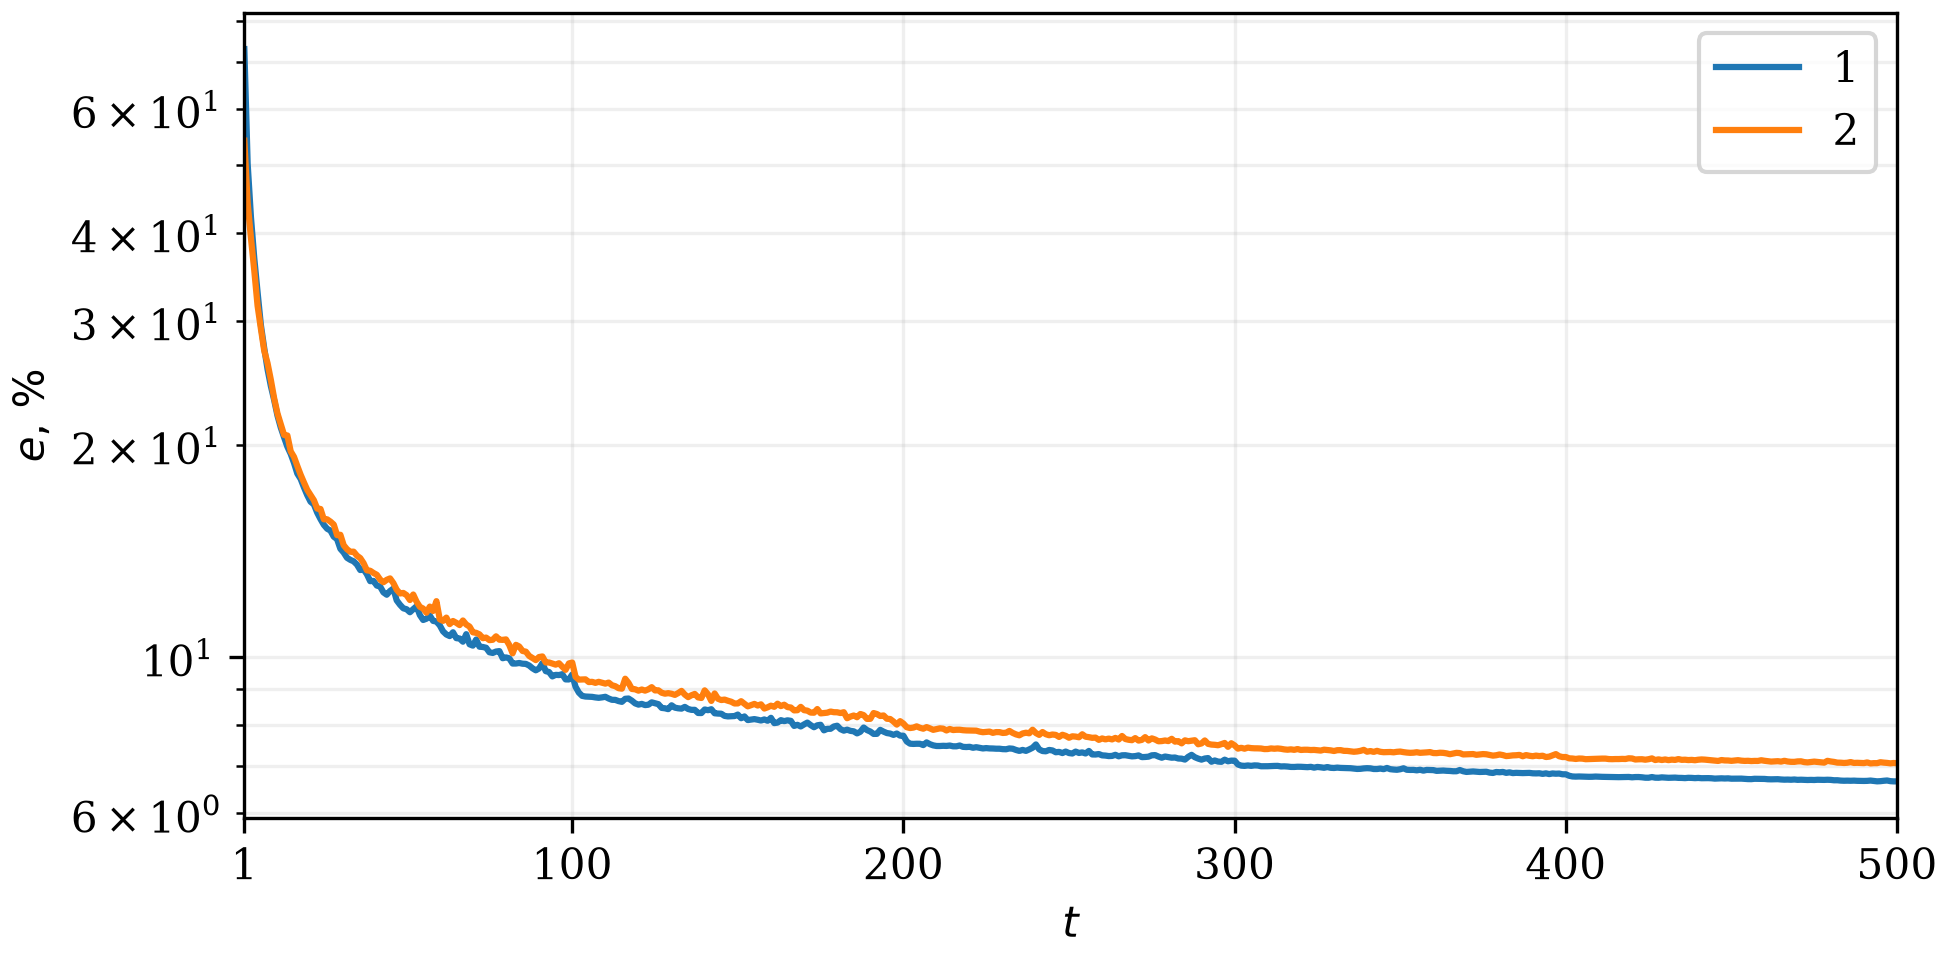
\includegraphics[width=0.85\linewidth]{images/figure1.png}
\caption{Изменение функции потерь в течение первых 500 эпох: 1 --- обучающая выборка, 2 --- валидационная выборка; $t$ --- номер эпохи, $e$ --- значение функции потерь в процентах.}
\label{fig:training}
\end{figure}

% Тестовые ошибки нейросети добавить только после оценки checkpoint из первых 500 эпох.
На той же валидационной выборке средняя узловая ошибка проекции решения на выбранные базисы при \(R=71\) составила около \(0{,}970\%\). Это значение меньше наименьшей ошибки нейросетевого приближения за рассматриваемые 500 эпох. Разложение ошибки~\eqref{eq:error_decomposition} позволяет отделить ошибку проекции от ошибки определения коэффициентов; исследование влияния изменения ранга требует дополнительных расчётов.

Раздельное влияние нормировки, ранга, функции потерь и длительности обучения требует дополнительных экспериментов при фиксированных остальных параметрах.

Результаты относятся к новым комбинациям включений в пределах заданных 24 позиций. Перенос на произвольные геометрии, другие сетки и волновые числа вне диапазона~\eqref{eq:ranges} в данном эксперименте не проверяется. Исследование сходимости конечно-элементного решения по сетке и измерение ускорения относительно прямого решателя также требуют отдельного расчёта.

\section{ЗАКЛЮЧЕНИЕ}
Рассмотрена схема приближённого решения задачи рассеяния, объединяющая конечно-элементное формирование данных, SVD-представление полей и обучение спектрального отображения между коэффициентами. Выбор числа мод по валидационной ошибке позволяет согласовать размер модели с заданной точностью восстановления. Сопоставление ошибки проекции и валидационной ошибки нейросети указывает на необходимость дальнейшего исследования точности отображения между коэффициентами. Тестовую оценку модели, выбранной в пределах 500 эпох, предстоит выполнить отдельно.

Для дальнейшего исследования целесообразно сравнить несколько рангов при одинаковом числе обучающих шагов, оценить разброс результатов при разных начальных приближениях и проверить зависимость точности от разрешения сетки.

\begin{thebibliography}{9}
\bibitem{li2020}
Li Z., Kovachki N., Azizzadenesheli K., Liu B., Bhattacharya K., Stuart A., Anandkumar A.
Fourier Neural Operator for Parametric Partial Differential Equations.
2020. \href{https://arxiv.org/abs/2010.08895}{arXiv:2010.08895}.
\bibitem{fanaskov2022}
Fanaskov V., Oseledets I.
Spectral Neural Operators.
2022. \href{https://arxiv.org/abs/2205.10573}{arXiv:2205.10573}.
\bibitem{halko2011}
Halko N., Martinsson P.-G., Tropp J.\,A.
Finding Structure with Randomness: Probabilistic Algorithms for Constructing Approximate Matrix Decompositions.
SIAM Review. 2011. Vol.~53, No.~2. P.~217--288.
\href{https://doi.org/10.1137/090771806}{doi:10.1137/090771806}.
\end{thebibliography}
\end{document}
